\documentclass{beamer}

\usepackage[utf8]{inputenc}

\usepackage{amsmath}
\usepackage{amssymb}
\usepackage{amsthm}
\usepackage{amsfonts}
\usepackage{xspace}
\usepackage{tabularx,booktabs,multirow}

\usepackage{hyperref}
\usepackage{url}

\usepackage{tikz}
\usepackage{color}
\usetikzlibrary{calc,shapes,fadings,automata,backgrounds,petri,shapes,decorations,decorations.pathmorphing,decorations.pathreplacing}


%%%%%%%%%% Tool Names %%%%%%%%%%%%
\newcommand{\nest}{\mathit{nest}_\nu}
\newcommand{\depth}{\mathit{depth}}
\newcommand{\set}[1]{\left\{#1\right\}}
\newcommand{\pset}[2]{\set{\,#1\mid#2\,}}
\newcommand{\process}{\mathcal{P}}
\newcommand{\Reach}{\mathit{Reach}}
\newcommand{\subgraph}{\mathrel{\hookrightarrow}}
\newcommand{\picasso}{\textsc{Picasso}\xspace}
\newcommand{\this}{\ensuremath{\mathit{this}}}
\newcommand{\st}{\ensuremath{\mathit{st}}}
\newcommand{\new}{\ensuremath{\mathbf{new}}}
\newcommand{\assume}{\ensuremath{\mathbf{assume}}}
\newcommand{\throw}{\ensuremath{\mathbf{throw}}}

\mode<presentation>
{
  \usetheme{Warsaw}
%  \useoutertheme{mysplit}
}
% Remove the navigation bar
\setbeamertemplate{navigation symbols}{}

\graphicspath{{./imgs/}}

\title[DPI]{Dynamic Package Interface}

\author{Damien Zufferey}

\institute{
  IST Austria
}
\date{joint work with Shahram Esmaeilsabzali, Rupak Majumdar, and Thomas Wies.}

\begin{document}

% Title
\frame[plain]{\titlepage}

\begin{frame}[fragile]
  \frametitle{State machine interface for single object}
  Example: Spin lock 
  \begin{columns}
    \column{0.5\linewidth}
{\scriptsize
\begin{verbatim}
void lock(spinlock *lock)
{
  while (1)
  {
    if (!xchg_32(lock, BUSY)) return;
    while (*lock) cpu_relax();
  }
}

void unlock(spinlock *lock)
{
  barrier();
  assert(*lock)
  *lock = 0;
}
\end{verbatim}
}
    \column{0.5\linewidth}
  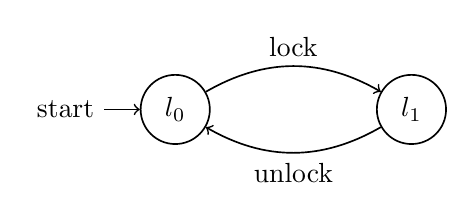
\begin{tikzpicture}[->,auto, node distance=3cm, semithick]
    \node [state,initial] (pi0) {$l_0$};
    \node [state] (pi1) [right of=pi0] {$l_1$};
    \path
    (pi0) edge [bend left] node { lock } (pi1)
    (pi1) edge [bend left] node { unlock } (pi0)
    ;
  \end{tikzpicture}
  \end{columns}
\end{frame}

\begin{frame}
  \frametitle{Dynamic package interface}

  Extend state-machine interface to group of objects.

  \vspace{3ex}
  There can be an unbounded number of objects.

  For the sake of simplicity, the example are shown in a non-concurrent setting.

\end{frame}

\begin{frame}[fragile]
  \frametitle{Example: Sets and Iterators}
  \begin{columns}
    \column{0.5\linewidth}
{\footnotesize
\begin{verbatim}
class Set {
  protected int sver, size;
  public Set() {
    sver := size := 0;
  }
  public void add(int elem) {
    if (!duplicate) {
      sver++; size++;
    }
  }
  protected void delete(int pos) {
    sver++; size--;
  }
  public Iterator iterator() {
    return (new Iterator(this));
  }
}
\end{verbatim}
}
    \column{0.5\linewidth}
{\footnotesize
\begin{verbatim}
class Iterator {
  int iver, pos;
  Set it_of;
  protected Iterator(Set s) {
    it_of := s; pos := 0;
    iver := s.sver;
  }
  public int next() {
    if (iver == S.sver) then pos++;
    else throw new Exception();
  }
  public void remove() {
    if (iver == S.sver) then {
      it_of.delete(pos);
      iver := S.sver;
    } else {
      throw new Exception();
} } }
\end{verbatim}
}
  \end{columns}

\end{frame}

\begin{frame}
  \frametitle{Simple OO model: syntax}
  A state is $(O, \this, q, v, \st)$ where
  \begin{itemize}
  \item $O$ is the set of objects
  \item $q$ is the control-state
  \item $v$ is the stack (\this\ + $q$)
  \item \st is the store
  \end{itemize}

  A method is a CFA with the operations on the edges:
  \begin{itemize}
  \item $\this.x := \ldots$ 
  \item $\this.m(\ldots)$
  \item $\new\ O(\ldots)$
  \item $\assume(\ldots)$
  \item $\throw\ \ldots$
  \end{itemize}
\end{frame}

\begin{frame}
  \frametitle{Simple OO model: semantics}
  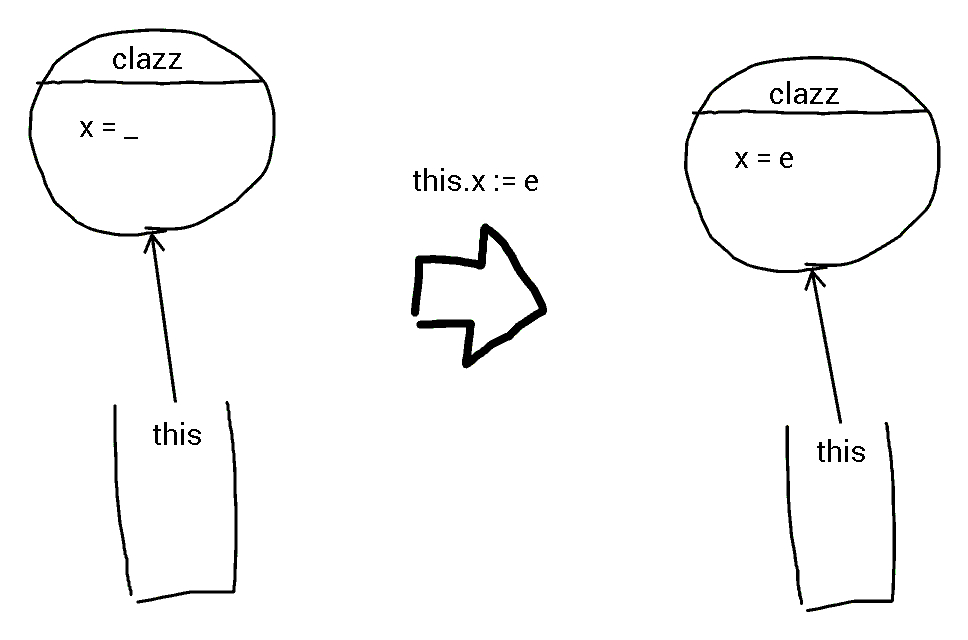
\includegraphics[width=\linewidth]{assign}
\end{frame}

\begin{frame}
  \frametitle{Simple OO model: semantics}
  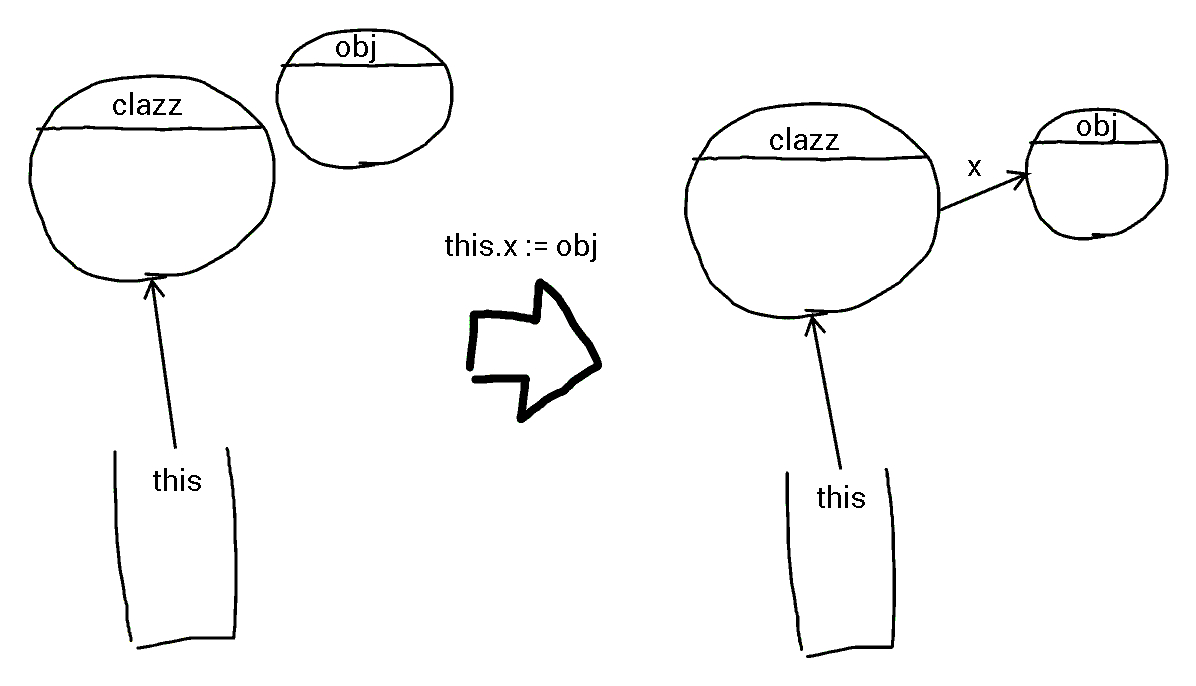
\includegraphics[width=\linewidth]{assign_obj}
\end{frame}

\begin{frame}
  \frametitle{Simple OO model: semantics}
  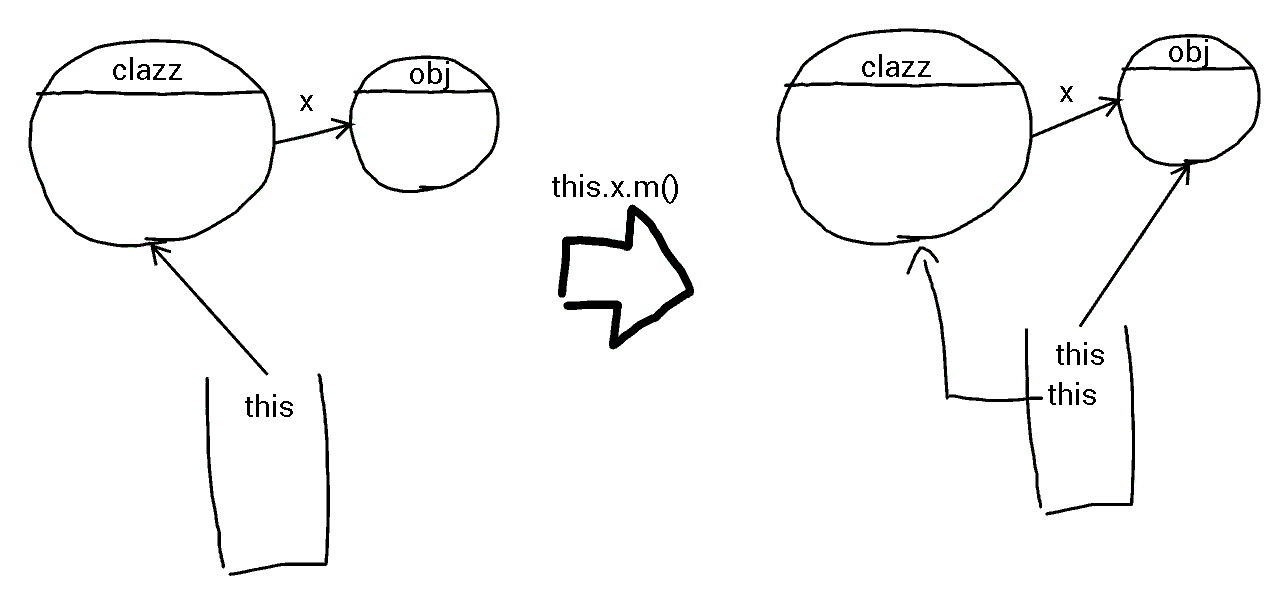
\includegraphics[width=\linewidth]{call}
\end{frame}

\begin{frame}
  \frametitle{Simple OO model: semantics}
  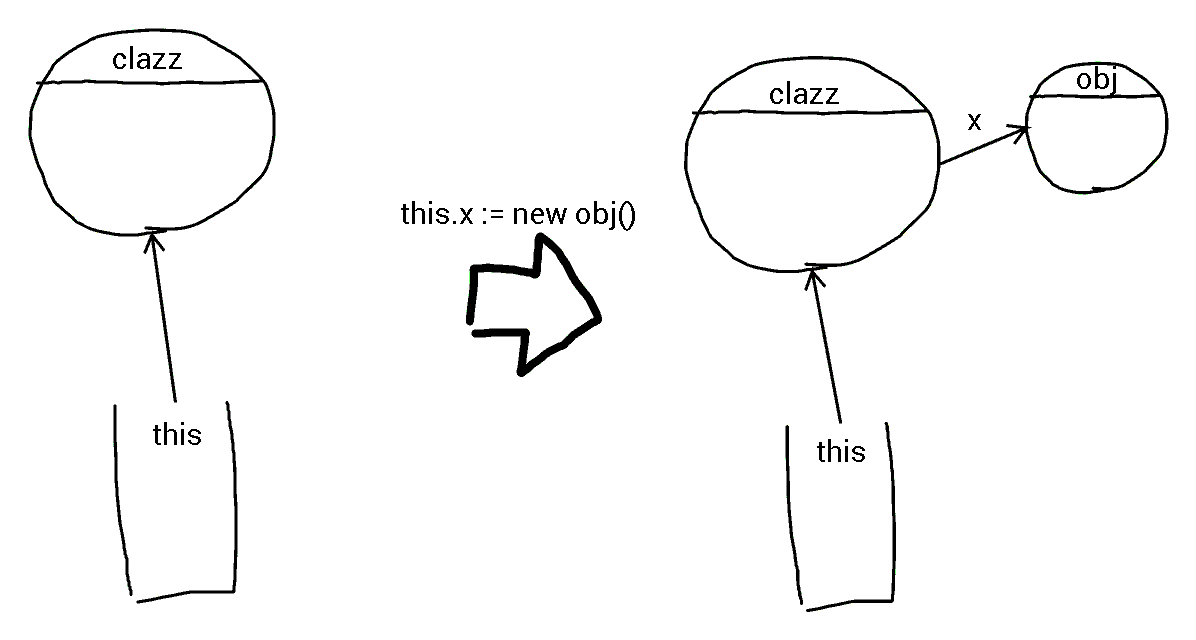
\includegraphics[width=\linewidth]{new}
\end{frame}

\begin{frame}
  \frametitle{Simple OO model: semantics}
  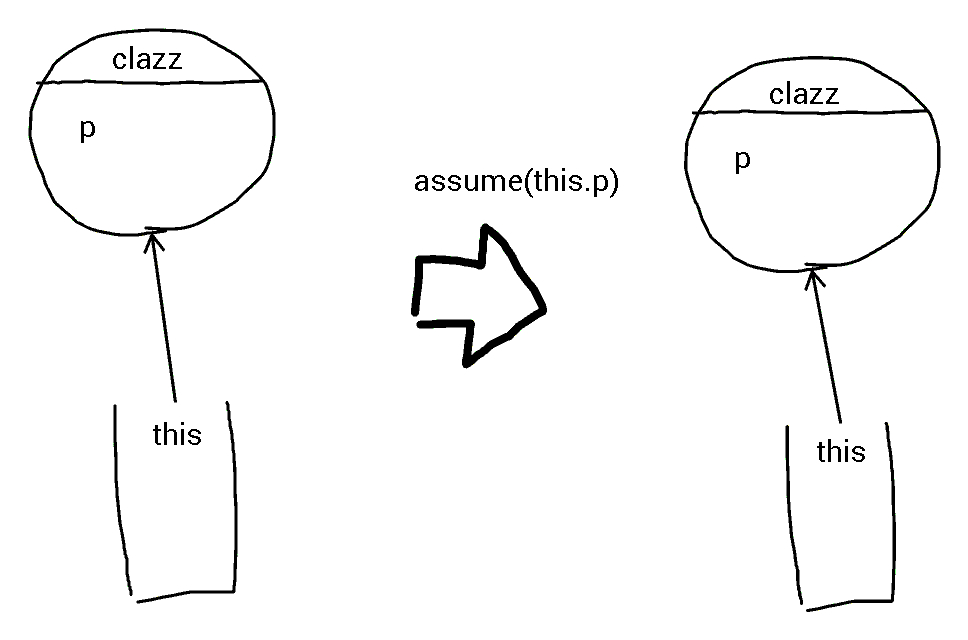
\includegraphics[width=\linewidth]{assume_pass}
\end{frame}

\begin{frame}
  \frametitle{Simple OO model: semantics}
  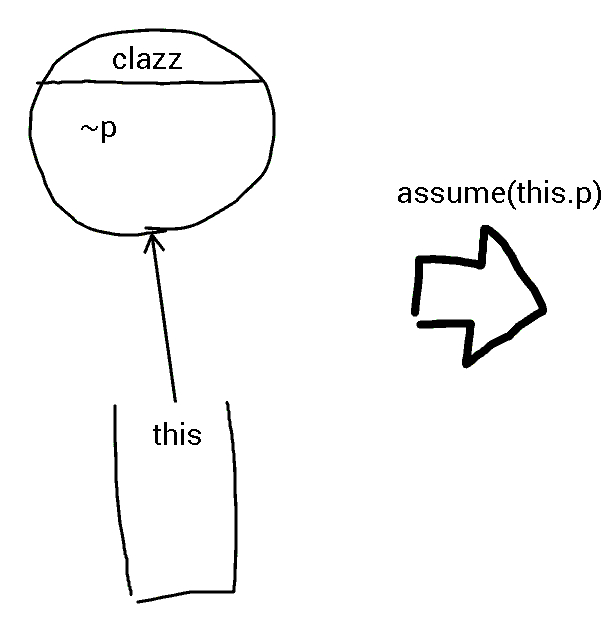
\includegraphics[width=0.6\linewidth]{assume_fail}
\end{frame}

\begin{frame}
  \frametitle{Simple OO model: semantics}
  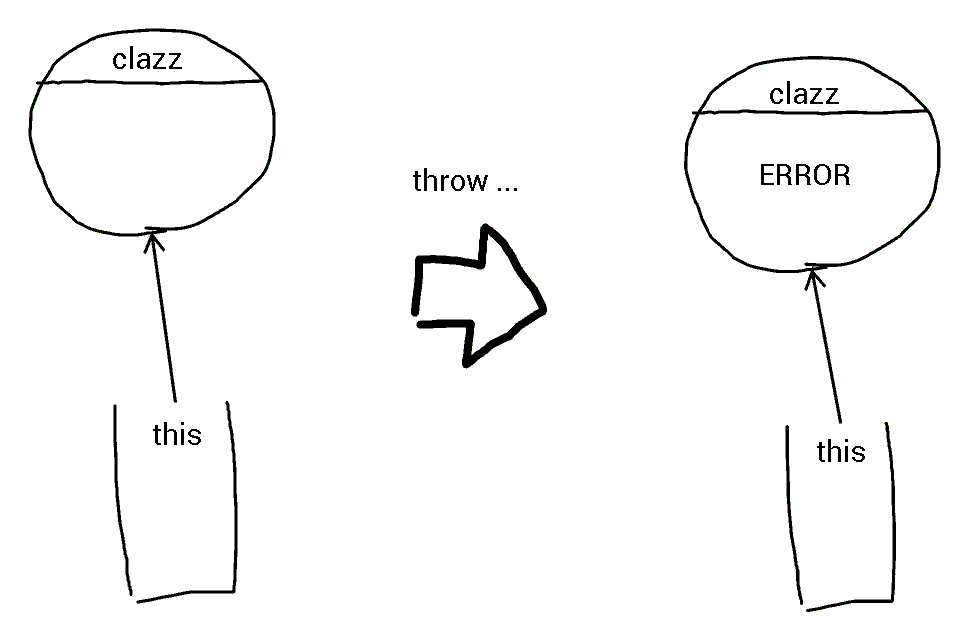
\includegraphics[width=\linewidth]{throw}
\end{frame}

\begin{frame}
  \frametitle{Predicate abstraction}

  We want interfaces with finite representation.\\
  $\mbox{}\ \ \Rightarrow$ cannot remember everything.\\
  $\mbox{}\ \ \ \ \Rightarrow$ predicate abstraction.

  \vspace{4ex}

  Two classes of predicates:
  \begin{itemize}
  \item unary predicate:\\
    empty for {\tt Set} ({\tt size = 0})
  \item binary predicates:\\
    sync for {\tt Iterator} ({\tt iver = it\_of.sver})\\
    mover for {\tt Iterator} ({\tt pos < it\_of.size})\\
  \end{itemize}

\end{frame}

\begin{frame}
  \frametitle{Predicate abstraction}
  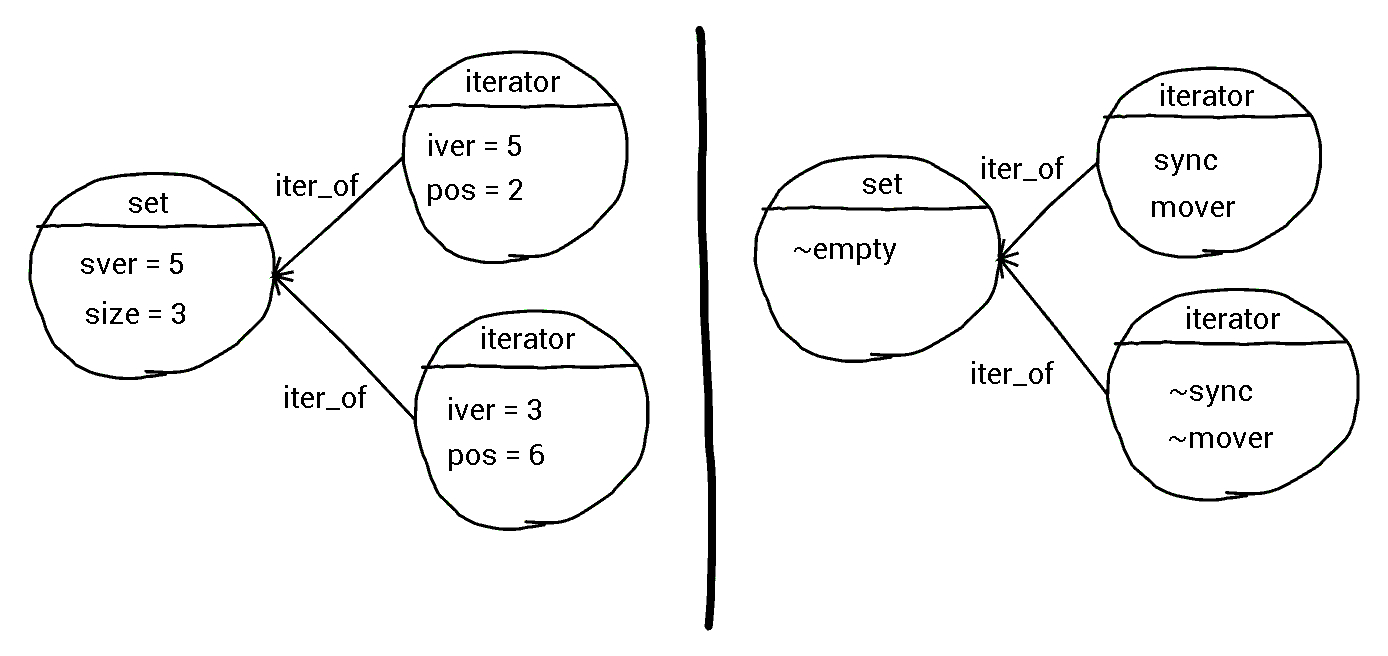
\includegraphics[width=\linewidth]{abstraction}
\end{frame}

\begin{frame}
  \frametitle{Abstract post}
  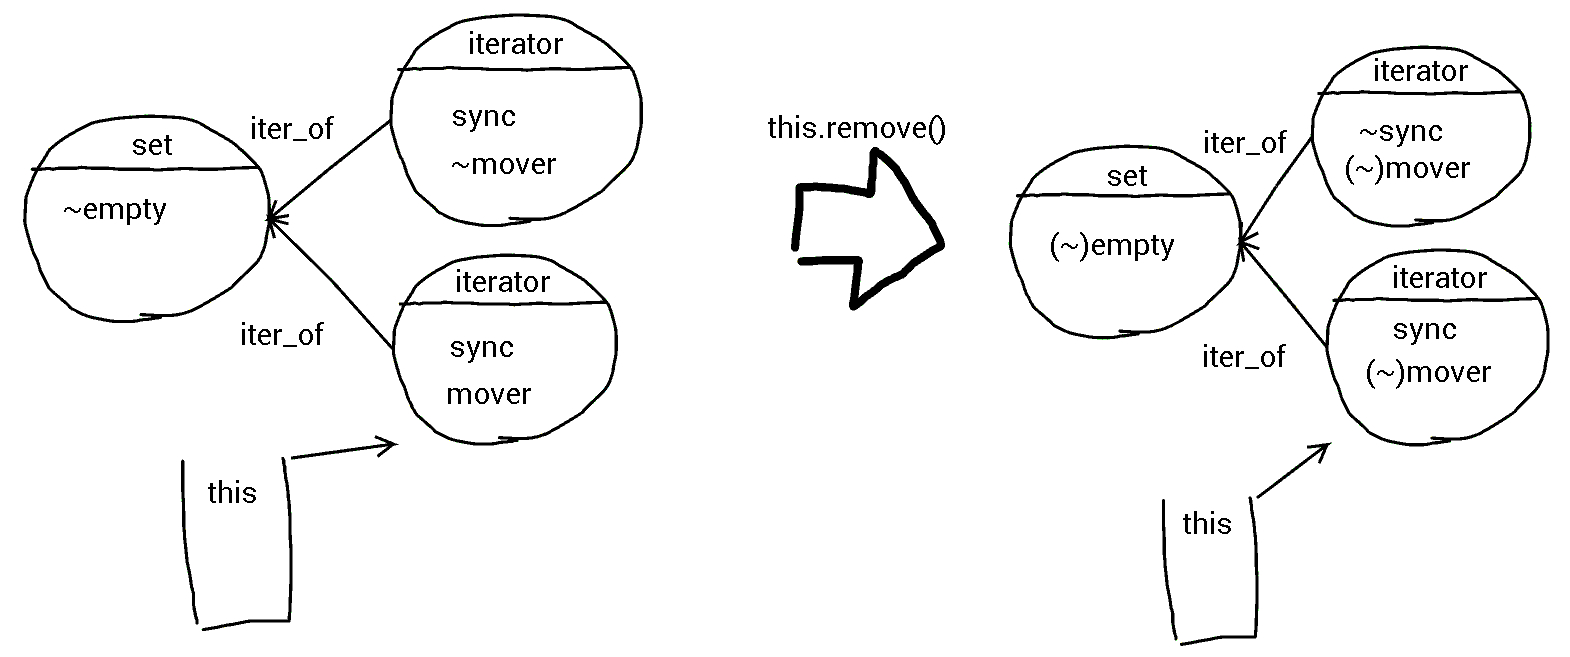
\includegraphics[width=\linewidth]{abs_post}

  \vspace{1ex}

  The new predicates can be computed testing (for empty in $set$):
  \begin{eqnarray*}
    \varphi(set,\this) & \Rightarrow & wp(\text{\this.remove}, \text{empty}_{set'}) \\
    \varphi(set,\this) & \Rightarrow & wp(\text{\this.remove}, \neg\text{empty}_{set'})
  \end{eqnarray*}
  $\varphi$ encodes the graph structure as a formula.
\end{frame}

\begin{frame}
  \frametitle{Representing a DPI}
  State-machine interfaces are automata.
  We try follow that idea with DPI.

  \vspace{2ex}

  \begin{itemize}
  \item What are the states ?
  \item What is the alphabet ?
  \end{itemize}

\end{frame}

\begin{frame}
  \frametitle{The states}
  States are graphs.
  Nodes represent equivalence classes of objects.

  \vspace{1ex}

  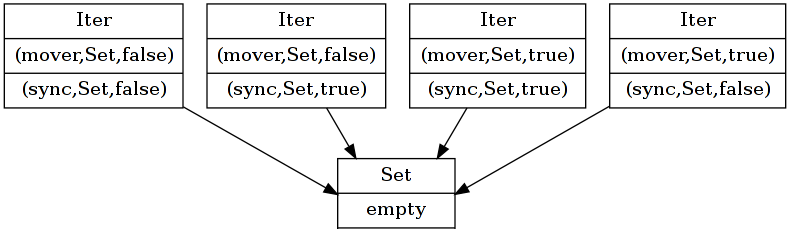
\includegraphics[width=\linewidth]{state.png}

  \vspace{2ex}

  To have a finite number of states in the DPI we require that:
  \begin{itemize}
  \item longest acyclic path in any graph (undirected) is bounded (enforced by a sufficient syntactic restriction).
  \item there are a finite number of labels (predicate abstraction)
  \item stratified method call (bounded stack)
  \end{itemize}

\end{frame}

\begin{frame}
  \frametitle{The transitions}
  \begin{minipage}{0.48\linewidth}
  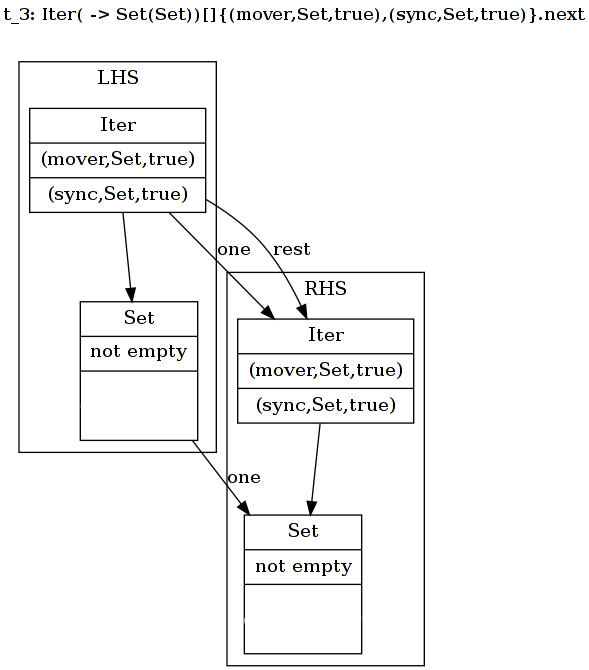
\includegraphics[scale=0.3]{transition.png}
  \end{minipage}
  \begin{minipage}{0.5\linewidth}
  Similar to state-machine interfaces we need an object (\this) + method name.

  \vspace{3ex}

  Additionally, the transition has a mapping of equivalence classes in the pre-state to the post-state.
  The systems are monotonic, so any equivalence classes which is not in the mapping is unchanged.
  \end{minipage}
\end{frame}

\begin{frame}
  \frametitle{Under the hood: depth-bounded systems}

  Monotonicity + the conditions on the graph $\Rightarrow$ DBS

  \vspace{3ex}

  Graphs of equivalence classes are ideals in the state space.
  By a strange coincidence we had a paper about ``Ideal abstraction for WSTS''.
  How convenient!

  \vspace{3ex}

  The last element needed to compute a DPI: the \emph{covering set}.
  
  \vspace{1ex}

  Nice properties of the covering set:
  \begin{itemize}
  \item has a compact representation (finite union of ideals)
  \item is an inductive invariant (subsumes all the system's behaviors)
  \end{itemize}
\end{frame}

\begin{frame}
  \frametitle{Extracting the DPI}
  \begin{itemize}
  \item compute the covering set and the DBS
  \item apply the post operator once more
  \item track each transition to get the DPI
  \end{itemize}

  \vspace{2ex}

  Show \picasso output for the Set and Iterators example.
\end{frame}

\begin{frame}
  \frametitle{How to use a DPI}

  Unfortunately, a DPI cannot be used out of the box.

  Why? the DPI is \alert{saturated}, the initial state of the system is \alert{empty}.

  \vspace{2ex}

  
  If we know in which equivalence classes the objects belongs, the DPI tells us how to update the state.
  Some bookkeeping is needed.

\end{frame}

\begin{frame}
  \frametitle{Conclusion}

  We presented:
  \begin{itemize}
  \item DPI as a generalisation of state-machine interfaces to groups of interacting objects.
  \item Abstraction to compute sound DPI.
  \end{itemize}

  \vspace{3ex}

  Future work:
  \begin{itemize}
  \item Feasibility study for the use of DPI (bookkeeping part).
  \end{itemize}

\end{frame}

\end{document}
